\subtop{Knickminimierung in orthogonalen Layouts}{-1.075}
\vspace*{-0.5\baselineskip}\\
Das Knickminimierungsproblem (allgemein) ist $\mathcal{NP}$-schwer.
\begin{description}[itemsep=-1pt]
	\item[orthogonale Beschreibung $(H)$] keine Kantenlängen, keine Positionen für Knoten\\
	eine Folge von Facettenbeschreibungen $H(f),~f\in \mathcal{F}$ mit Elementen $(e,\delta,x)$ definiert durch
	\begin{itemize}[itemsep=-2pt]
		\item $e\in E$
		\item $\delta$ eine Folge aus $\{0,1\}$, $0$ kodiert einen $\frac{\pi}{2}$ Knick, $1$ einen $\frac{3\pi}{2}$
		\item $x$ ein Winkel aus $\{0,\frac{\pi}{2},\pi,\frac{3\pi}{2}\}$
	\end{itemize}
	$H$ ist korrekt, falls
		\begin{description}[itemsep=-2pt]
			\item[O1] Es gibt eine planare Einbettung, die $H$ entspricht
			\item[O2] $(e,\delta_1,x_1),(e,\delta_2,x_2)\\
			\Rightarrow \delta_2$ entsteht aus $\delta_1$ durch kippen jedes einzelnen Bits von $\delta_1$ und umkehren der Folge $\delta_1$
			\item[O3] $|\delta|_0$, $|\delta|_1$ sind die Anzahl der $0/1$ in $\delta$\\
			für $r=(e,\delta,x)$ gilt $\mathcal{C}(r)=|\delta|_0-|\delta|_1+(2-\frac{2x}{\pi})\\
			\Rightarrow \sum\limits_{r\in H(f)}\mathcal{C}(r)=\left\{
				\begin{array}{rl}
					4&f\in \mathcal{F}\setminus\{f_0\}\\
					-4&f=f_0
				\end{array}
			\right.$
			\item[O4] $\forall v\in V$ ist die Summe der Winkel bei $v$ gleich $2\pi$
		\end{description}
		\example{\text{orthogonale Beschreibung}}{
			\ \\
			\vspace*{-\baselineskip}
			\begin{minipage}{0.5\textwidth}
				\usetikzlibrary{positioning,patterns,calc,arrows}

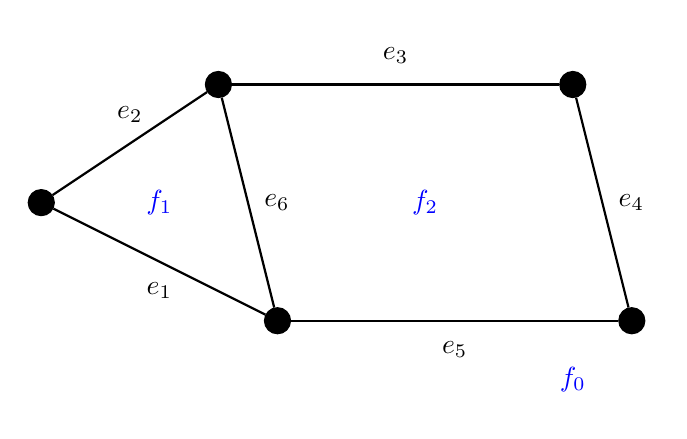
\begin{tikzpicture}[every node/.style={draw,fill,circle},node distance=0cm,scale=0.75]

\node(1) at (0,0) {};
\node(2) at (3,2) {};
\node(3) at (4,-2) {};
\node(4) at (9,2) {};
\node(5) at (10,-2) {};

\foreach[count=\c] \x/\y/\p in {1/3/below,1/2/above,2/4/above,4/5/right,5/3/below,2/3/right}
	\draw[-,thick](\x)to node[\p,draw=none,fill=none] {$e_{\c}$}(\y);

\node[draw=none,fill=none,color=blue] at (2,0) {$f_1$};
\node[draw=none,fill=none,color=blue] at (6.5,0) {$f_2$};
\node[draw=none,fill=none,color=blue] at (9,-3) {$f_0$};

\end{tikzpicture}
			\end{minipage}
			\begin{minipage}{0.5\textwidth}
				$\begin{array}{rcl}
					f_0&:&(e_1,11,\ph),(e_5,111,\dph),\\
					&&(e_4,\emptyset,\pi),(e_3,\emptyset,\pi),(e_2,\emptyset,\ph)\\
					&&\\
					f_1&:&(e_1,00,\dph),(e_2,\emptyset,\ph),(e_6,00,\pi)\\
					&&\\
					f_2&:&(e_5,000,\ph),(e_6,11,\ph),\\
					&&(e_3,\emptyset,\pi),(e_4,\emptyset,\ph)
				\end{array}$
			\end{minipage}
		}
	\item[orthogonales Layout] feste Positionen und somit auch Kantenlängen für alle Teile des Graphen
\end{description}
\subsection{Knickminimierung mit vorgegebener Einbettung}
\usetikzlibrary{positioning,arrows}

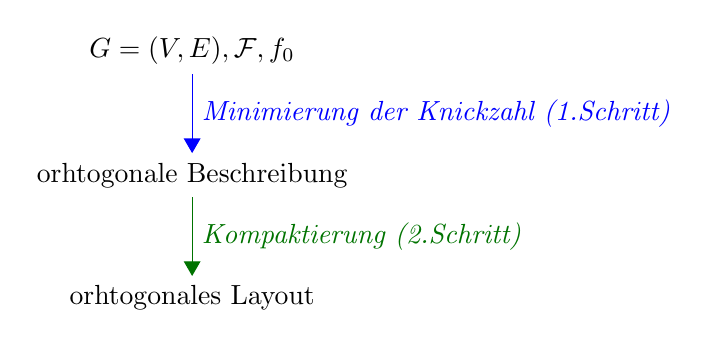
\begin{tikzpicture}[]

\node (0) at (0,0) {$G=(V,E),\mathcal{F},f_0$};
\node (1) [below=of 0] {orhtogonale Beschreibung};
\node (2) [below=of 1] {orhtogonales Layout};

\draw[->,>=triangle 60,color=blue](0)to node[right] {\textit{Minimierung der Knickzahl (1.Schritt)}}(1);
\draw[->,>=triangle 60,color=green!45!black](1)to node[right] {\textit{Kompaktierung (2.Schritt)}}(2);
\end{tikzpicture}\\
\vspace*{-2\baselineskip}
\subsubsection{Schritt 1: orthogonale Beschreibung}
\begin{description}
	\item[Definition des Flussnetzwerks $N(G)=((W,A),l,u,b,cost)$]\ \\\vspace*{-\baselineskip}
		\begin{eqnarray*}
			W&=&V\cup \mathcal{F}\\
			A&=&\{(v,f)\in V\times \mathcal{F}, v\text{ inzident zu }f\}\\
			&&\cup \{(f,g)\in\mathcal{F},~f\text{ und }g\text{ haben gemeinsame Kante}\}\\
			b(v)&=&4\ph\Rightarrow 4,~\forall v\in V\\
			b(f)&=&-2(d_G(f)-2)\ph\Rightarrow -2(d_G(f)-2),~\forall f\in\mathcal{F}\setminus\{f_0\}\\
			b(f_0)&=&-2(d_G(f)+2)\ph\Rightarrow -2(d_G(f)+2)
		\end{eqnarray*}
\end{description}
\topbreak
\vspace*{-3.5\baselineskip}
\begin{description}
	\item[]\ \\ \begin{eqnarray*}
				l(v,f)&=&1,~l(f,g)~=~0\\
				u(v,f)&=&4,~u(f,g)~=~\infty\\
				cost(v,f) &=&0, cost(f,g)~=~1
			\end{eqnarray*}
		Eine Flusseinheit entspricht einem $\ph$-Winkel/-Knick
\end{description}

\begin{itemize}[itemsep=-1pt]
	\item $N(G)=((W,A),l,u,b,cost)$ ist ein Flussnetzwerk (Beweis durch Satz von Euler)
	\item zu jedem planaren Graph mit $\Delta(G)\leq 4$ und kombinatorischer Einbettung existiert genau eine orthogonale Beschreibung mit $k$ Knicken, wenn es einen Fluss $x$ in $N(G)$ mit $k$ Kosten gibt
		\vspace*{-\baselineskip}\Proof {\color{red}\textbf{TODO}}%TODO
\end{itemize}

\subsubsection{Schritt 2: Kompaktierung}
\begin{itemize}[itemsep=-1pt]
	\item betrachten den Spezialfall mit der Eigenschaft, dass alls Facetten in $H(G)$ Rechtecke sind
	\item zur Konstruktion wird ein Flussnetzwerk verwendet
	\item für den Spezialfall kann garantiert werden: das konstruierten Layout hat:
		\begin{enumerate}
			\item minimale Gesamtkantenlänge
			\item minimale Fläche
		\end{enumerate}
	\item Konstruktion von zwei Flussnetzwerken ($N_{ver},N_{hor}$) mit $cost(a)=1, l(a)=1, u(a)=\infty$\\\\
		\begin{minipage}{0.48\textwidth}
			\begin{center}
			$N_{ver}=((W_{ver},A_{ver}),s,t\in W_{ver},l,u,cost)$\\
			\vspace*{2cm}
			\usetikzlibrary{positioning,patterns,calc,arrows}

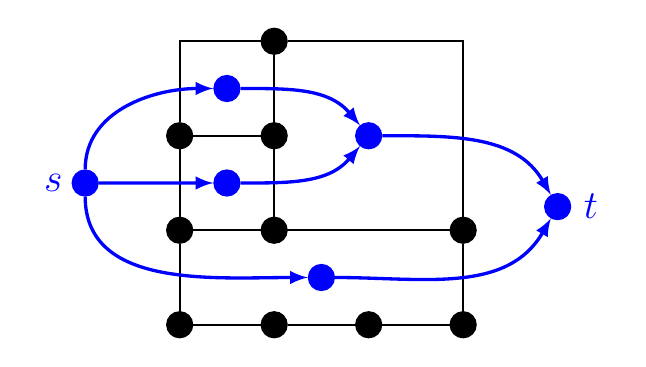
\begin{tikzpicture}[every node/.style={draw,fill,circle},node distance=0cm,scale=0.6]

\node(0) at (0,0) {};
\node(1) at (2,0) {};
\node(2) at (4,0) {};
\node(3) at (6,0) {};
\node(4) at (6,2) {};
\node(5) at (2,2) {};
\node(6) at (0,2) {};
\node(7) at (0,4) {};
\node(8) at (2,4) {};
\node(9) at (2,6) {};
\node[color=blue](f1) at (1,3) {};
\node[color=blue](f2) at (3,1) {};
\node[color=blue] (s) at (-2,3) {};
\node[color=blue] (t) at (8,2.5) {};
\node[color=blue](f3) at (4,4) {};
\node[color=blue](f4) at (1,5) {};
\node[left=of s,draw=none,fill=none,xshift=0.1cm,color=blue] {\Large$s$};
\node[right=of t,draw=none,fill=none,xshift=-0.1cm,color=blue] {\Large$t$};


\foreach \x/\y in {0/1,1/2,2/3,3/4,4/5,5/6,6/7,7/8,8/9,9/7,0/6,5/8,9/4}{
	\draw[thick](\x)-|(\y);
}
\draw[->,>=latex,very thick,color=blue] (s) to [out=270,in=180](f2);
\draw[->,>=latex,very thick,color=blue] (s) to(f1);
\draw[->,>=latex,very thick,color=blue] (s) to[out=90,in=180](f4);
\draw[->,>=latex,very thick,color=blue](f2)to[out=0,in=240](t);


\draw[->,>=latex,very thick,color=blue](f1)to[out=0,in=230](f3);
\draw[->,>=latex,very thick,color=blue](f4)to[out=0,in=130](f3);
\draw[->,>=latex,very thick,color=blue](f3)to[out=0,in=120](t);

\end{tikzpicture}
			\vspace*{1.5cm}
			\end{center}
		\end{minipage}
		\begin{minipage}{0.48\textwidth}
			\begin{center}
			$N_{hor}=((W_{hor},A_{hor}),s,t\in W_{hor},l,u,cost)$\\
			\vfill
			\usetikzlibrary{positioning,patterns,calc,arrows}

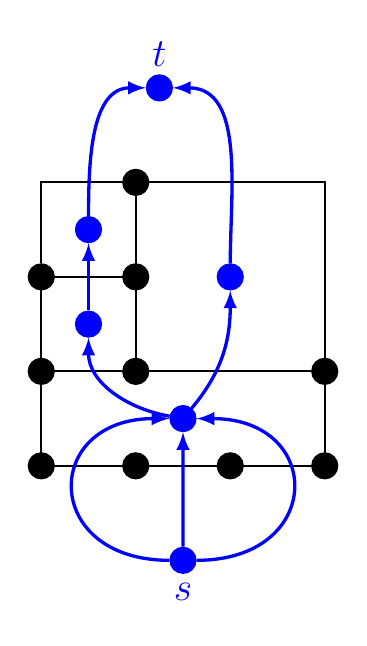
\begin{tikzpicture}[every node/.style={draw,fill,circle},node distance=0cm,scale=0.6]

\node(0) at (0,0) {};
\node(1) at (2,0) {};
\node(2) at (4,0) {};
\node(3) at (6,0) {};
\node(4) at (6,2) {};
\node(5) at (2,2) {};
\node(6) at (0,2) {};
\node(7) at (0,4) {};
\node(8) at (2,4) {};
\node(9) at (2,6) {};
\node[color=blue](f1) at (1,3) {};
\node[color=blue](f2) at (3,1) {};
\node[color=blue](s) at (3,-2) {};
\node[color=blue](t) at (2.5,8) {};
\node[color=blue](f3) at (4,4) {};
\node[color=blue](f4) at (1,5) {};
\node[below=of s,draw=none,fill=none,yshift=0.1cm,color=blue] {\Large$s$};
\node[above=of t,draw=none,fill=none,yshift=-0.1cm,color=blue] {\Large$t$};


\foreach \x/\y in {0/1,1/2,2/3,3/4,4/5,5/6,6/7,7/8,8/9,9/7,0/6,5/8,9/4}{
	\draw[thick](\x)-|(\y);
}
\draw[->,>=latex,very thick,color=blue](s)to(f2);
\draw[->,>=latex,very thick,color=blue] (s) .. controls (0,-2) and (0,1) .. (f2);
\draw[->,>=latex,very thick,color=blue] (s) .. controls (6,-2) and (6,1) .. (f2);
\draw[->,>=latex,very thick,color=blue](f2)to[out=170,in=270](f1);
\draw[->,>=latex,very thick,color=blue](f2)to[out=50,in=270](f3);
\draw[->,>=latex,very thick,color=blue](f1)to(f4);
\draw[->,>=latex,very thick,color=blue](f4)to[out=90,in=180](t);
\draw[->,>=latex,very thick,color=blue](f3)to[out=90,in=0](t);
\end{tikzpicture}
			\end{center}
		\end{minipage}\\
	\vspace*{-3\baselineskip}
	\item \textbf{Beobachtungen:}
		\begin{itemize}
			\item alle Knicke liegen auf $f_0$
			\item wenn gegenüberliegende Seiten die Gleiche Länge zugewiesen bekommen, kann ein korrektes Layout konstruiert werden
		\end{itemize}
	\item für ganzzahlige Kantenbewertung $x_{ver},x_{hor}$ mit minimalen Kosten im entsprechenden Flussnetzwerk und orthogonaler Beschreibung, die nur aus Rechtecken besteht, gilt:
		\begin{enumerate}[itemsep=-1pt]
			\item $x_{ver},x_{hor}$ ist ein Fluss gdw. die Kantenlängen ein korrektes Layout induzieren\\
			\textbf{Begründung:} Äquivalenz der Flusserhaltungsbedingung und Layouteigenschaft (gegenüberliegende Seiten haben gleiche Länge)
			\item der Wert von $x_{ver}$ entspricht der Höhe des Layouts, $x_{hor}$ entspricht der Breite des Layouts\\
			\textbf{Begründung:} durch Konstruktion
			\item $x_{hor}+x{ver}$ entspricht der Gesamtkantenlänge des Layouts\\
			\textbf{Begründung:} durch Konstruktion
		\end{enumerate}
	\item[$\Rightarrow$] Flüsse mit minimalen ganzzahligen Kosten induzieren ein planares, orthogonales Gitterlayout mit minimaler Fläche und Gesamtkantenlänge
\end{itemize}
\topbreak
\vspace*{-2\baselineskip}
\subsubsection{Erweiterung auf den allgemeinen Fall}
\begin{description}
	\item[rectangular refinement von $H(G)$] ist eine orthogonale Beschreibung $H'(G')$ von $G$ mit
		\begin{itemize}
			\item $G'$ ist entstanden aus einer Sequenz der folgenden Operationen:
				\begin{itemize}
					\item Hinzufügen eines isolierten Knotens
					\item Hinzufügen von Knoten auf Kanten
					\item Hinzufügen von Kanten
				\end{itemize}
			\item die \glqq Teilbeschreibung\grqq durch $H'$ von $G$ ist die gleiche wie $H(G)$
			\item die Facetten von $H'(G')$ sind Rechtecke
			\item[$\Rightarrow$] man erhält eine Zeichnung von $G$ mithilfe einer Zeichnung von $G'$ (ohne hinzugefügte Elemente) 
		\end{itemize}
\end{description}
\begin{description}
	\item[1. Realisierung:] $G'=G,H'(G')=H(G)$
		\begin{itemize}
			\item Einfügen eines Knotens auf jedem Knick von $H(G)$
			\item Aktualisieren von $H'(G')$
		\end{itemize}
	\item[2. Facetten haben beliebige orthogonale Form:]\ \\\vspace*{-\baselineskip}
		\begin{enumerate}
			\item \textbf{innere Facetten:}\\
			\vspace*{-\baselineskip}
				\begin{minipage}{0.3\textwidth}
					\usetikzlibrary{positioning,patterns,calc,arrows}

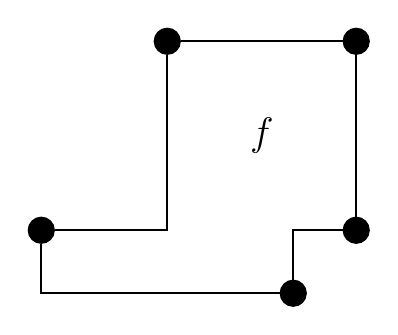
\begin{tikzpicture}[every node/.style={draw,fill,circle},node distance=0cm,scale=0.8]

\node(1) at (0,0) {};
\node(2) at (2,3) {};
\node(3) at (5,3) {};
\node(4) at (5,0) {};
\node(5) at (4,-1) {};

\foreach \x/\y in {1/2,2/3,3/4,4/5,5/1}{
	\draw[thick](\x)-|(\y);
}

\node[draw=none,fill=none]at(3.5,1.5){\Large$f$};

\end{tikzpicture}
				\end{minipage}
				{\Large{$\Longrightarrow$}}
				\begin{minipage}{0.4\textwidth}
					\usetikzlibrary{positioning,patterns,calc,arrows}

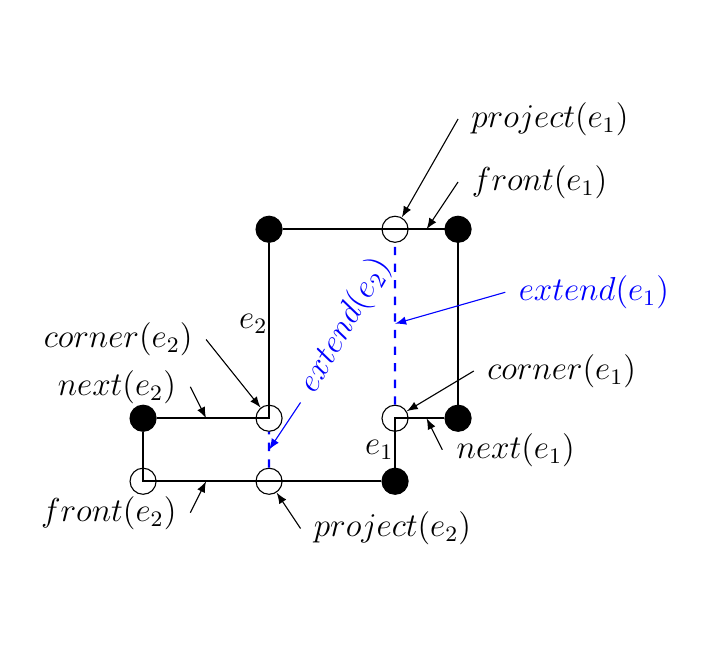
\begin{tikzpicture}[every node/.style={draw,fill,circle},node distance=0cm,scale=0.8]

\node(1) at (0,0) {};
\node(2) at (2,3) {};
\node(3) at (5,3) {};
\node(4) at (5,0) {};
\node(5) at (4,-1) {};

\node[fill=none](6) at (2,0) {};
\node[fill=none](7) at (4,0) {};
\node[fill=none](8) at (0,-1) {};
\node[fill=none](9) at (2,-1) {};
\node[fill=none](10) at (4,3) {};

\foreach \x/\y in {1/2,2/3,3/4,4/5,5/1}{
	\draw[thick](\x)-|(\y);
}
\foreach \x/\y in {9/6,7/10}{
	\draw[thick,dashed,color=blue](\x)--(\y);
}
\foreach[count=\c] \x/\y in {3.75/-0.5,1.75/1.5}{
	\node[fill=none,draw=none](e\c) at (\x,\y) {\large$e_{\c}$};
}
\foreach[count=\c] \x/\y/\e/\to/\a in {5.25/0.75/1/7/west,1/1.25/2/6/east}{
	\node[fill=none,draw=none,anchor=\a](c) at (\x,\y) {\large $corner(e_{\e})$};
	\draw[->,>=latex](c.\a)--(\to);
}
\foreach[count=\c] \x/\y/\e/\to/\a in {5/4.75/1/10/west,2.5/-1.75/2/9/west}{
	\node[fill=none,draw=none,anchor=\a](c) at (\x,\y) {\large $project(e_{\e})$};
	\draw[->,>=latex](c.\a)--(\to);
}
\foreach[count=\c] \x/\y/\e/\to/\tt/\a in {0.75/0.5/2/1/6/east,4.75/-0.5/1/7/4/west}{
	\node[fill=none,draw=none,anchor=\a](n) at (\x,\y) {\large $next(e_{\e})$};
	\draw[->,>=latex](n.\a)--($(\to)!0.5!(\tt)$);
}
\foreach[count=\c] \x/\y/\e/\to/\tt/\a/\r in {2.5/0.25/2/9/6/west/60,5.75/2/1/7/10/west/0}{
	\node[fill=none,draw=none,anchor=\a,color=blue,rotate=\r](e) at (\x,\y) {\large $extend(e_{\e})$};
	\draw[->,>=latex,color=blue](e.\a)--($(\to)!0.5!(\tt)$);
}
\foreach[count=\c] \x/\y/\e/\to/\tt/\a in {0.75/-1.5/2/9/8/east,5/3.75/1/3/10/west}{
	\node[fill=none,draw=none,anchor=\a](f) at (\x,\y) {\large $front(e_{\e})$};
	\draw[->,>=latex](f.\a)--($(\to)!0.5!(\tt)$);
}
\end{tikzpicture}
				\end{minipage}\\
				Ablauf:
					\begin{enumerate}
						\item Realisierung für jede Facette $f\in\mathcal{F}$
						\item für jede Kante $e$ in $H'(f)$ wird folgendes definiert:\\
							\begin{tabular}{rcl}
								$next(e$)&$:$&nächste Kante in $H'(f)$ (counterclockwise)\\
								$corner(e)$&$:$& gemeinsamer Knoten von $e$ und $next(e)$\\
								$turn(e)$&$:$&$\left\{\begin{array}{rcl}
									1&:&next(e)\text{ knickt nach links ab}\\
									0&:&next(e)\text{ knickt nicht ab}\\
									-1&:&next(e)\text{ knickt nach recht ab}
								\end{array}\right.$\\
								$front(e)$&$:$& erste Kante $e'$ in $H'(f)$ nach $e$, für die gilt:\\
								&& Summe der $turn$-Werte aller Kanten\\
								&& von \textit{\textbf{inklusiv}} $e$ bis \textit{\textbf{exklusiv}} $e'$ gleich $1$ ist
							\end{tabular}
						\item für $e$ mit $turn(e)=-1$ wird ein neuer Knoten $project(e)$ auf $front(e)$ sowie eine neue geradlinige Kante $estend(e)=(corner(e),project(e))$ eingefügt, Erweiterung von $H'(G')$ entsprechend
						\item falls $front(e)=front(e') \Rightarrow project(e)$  nach $project(e')$ eingefügt\\
						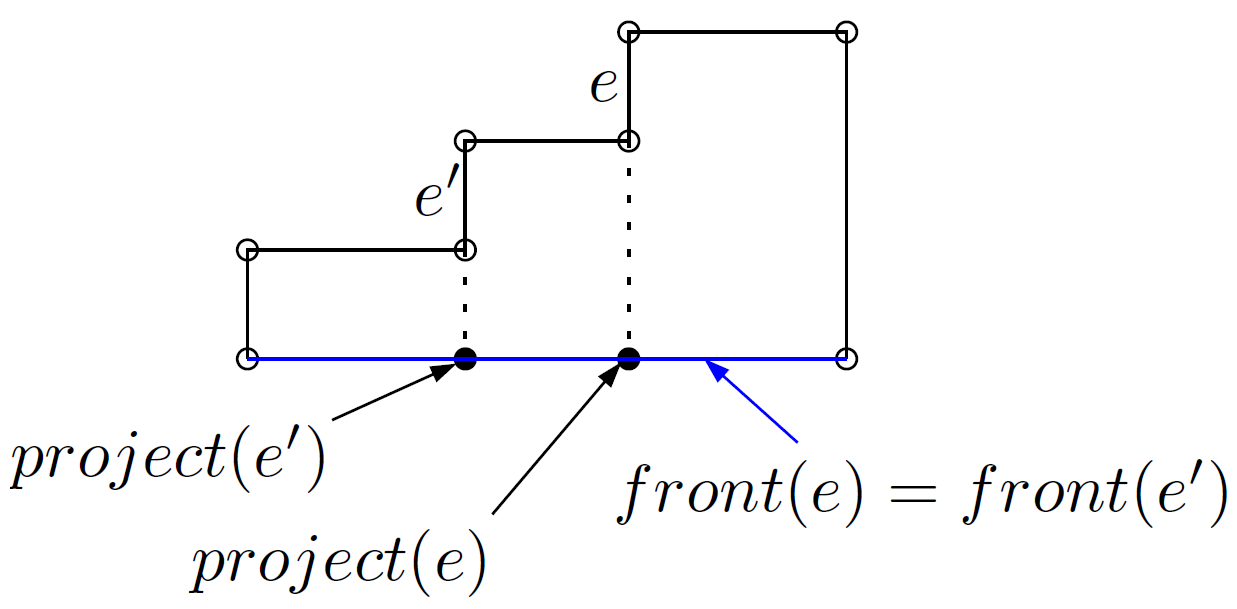
\includegraphics[height=2cm]{Pics/3_refinement-front.png}
					\end{enumerate}
		\end{enumerate}
\end{description}
\topbreak
\vspace*{-4\baselineskip}
\begin{description}
	\item[]\ \\
		\begin{enumerate}
		\setcounter{enumi}{1}
			\item \textbf{äußere Facette:} um $G$ wird ein minimales Rechteck gelegt, auf das die Knicke der äußeren Facette projiziert werden
		\end{enumerate}
	\item[Bemerkungen:]\ \\\vspace*{-\baselineskip}
		\begin{itemize}
			\item $k$ ist die Anzahl der Knicke in $H(G)\\
			\Rightarrow H'(G')$ hat $\BigO(n+k)$ Knoten\\
			$\Rightarrow H'(G')$ kann in $\BigO(n+k)$ konstruiert werden
			\item die Flussnetzwerke zu $H'(G')$ garantieren \textbf{nicht} mehr minimale Gesamtkantenlänge und minimale Fläche
			\item mit einem geeigneten Algorithmus für die Flussberechnung (minimale Kosten) kann zu planaren Graphen mit kombinatorischer Einbettung ein orthogonales Layout mit minimaler Knickzahl in $\BigO(n^{\frac{7}{4}}\cdot \log n)$ berechnet werden
		\end{itemize}
	\item[Erweiterung auf allgemeine Graphen:]\ \\\vspace*{-\baselineskip}
		ohne Gradbeschränkung (als Beispiel):\\
			\usetikzlibrary{positioning,patterns,calc,arrows}

\begin{tikzpicture}[node distance=0cm,scale=0.5]

\node (a) at (0,0) {
	\usetikzlibrary{positioning,patterns,calc,arrows}

\begin{tikzpicture}[every node/.style={draw,fill,circle},node distance=0cm,scale=0.5]
\node at (0,0) {};
\coordinate(1) at (-2.5,2) {};
\coordinate(2) at (2.5,-2) {};
\coordinate(3) at (0,3) {};
\coordinate(4) at (0,-3) {};
\coordinate(5) at (-3,-1) {};
\coordinate(6) at (3,1) {};
\draw  (1) edge (2);
\draw  (5) edge (6);
\draw  (3) edge (4);
\end{tikzpicture}
};
\node (b) at(13,0) {
	\usetikzlibrary{positioning,patterns,calc,arrows}

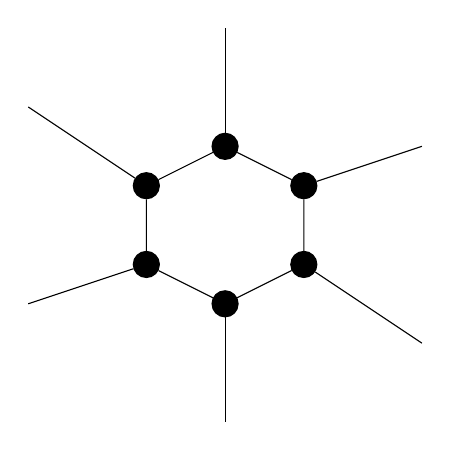
\begin{tikzpicture}[every node/.style={draw,fill,circle},node distance=0cm,scale=0.5]
\coordinate(1) at (-5,3) {} {};
\coordinate(2) at (5,-3) {} {};
\coordinate(3) at (0,5) {} {};
\coordinate(4) at (0,-5) {} {};
\coordinate(5) at (-5,-2) {} {};
\coordinate(6) at (5,2) {} {};

\node (v2) at (-2,1) {};
\node (v3) at (0,2) {};
\node (v4) at (2,1) {};
\node (v5) at (2,-1) {};
\node (v6) at (0,-2) {};
\node (v1) at (-2,-1) {};
\draw (v1) -- (v2) -- (v3) -- (v4) -- (v5) -- (v6) -- (v1);
\draw  (v1) edge (5);
\draw  (v2) edge (1);
\draw  (v3) edge (3);
\draw  (v4) edge (6);
\draw  (v5) edge (2);
\draw  (v6) edge (4);
\end{tikzpicture}
};
\node (c) at (26,0) {
	\usetikzlibrary{positioning,patterns,calc,arrows}

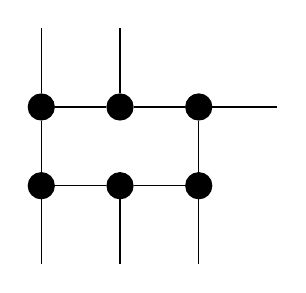
\begin{tikzpicture}[every node/.style={draw,fill,circle},node distance=0cm,scale=0.5]
\coordinate(1) at (-5,3) {} {};
\coordinate(2) at (-1,-3) {} {};
\coordinate(3) at (-3,3) {} {};
\coordinate(4) at (-3,-3) {} {};
\coordinate(5) at (-5,-3) {} {};
\coordinate(6) at (1,1) {} {};

\node (v2) at (-5,1) {};
\node (v3) at (-3,1) {};
\node (v4) at (-1,1) {};
\node (v5) at (-1,-1) {};
\node (v6) at (-3,-1) {};
\node (v1) at (-5,-1) {};
\draw (v1) -- (v2) -- (v3) -- (v4) -- (v5) -- (v6) -- (v1);
\draw  (v1) edge (5);
\draw  (v2) edge (1);
\draw  (v3) edge (3);
\draw  (v4) edge (6);
\draw  (v5) edge (2);
\draw  (v6) edge (4);
\end{tikzpicture}
};

\draw[->,>=latex,line width=3pt](a)--(b);
\draw[->,>=latex,line width=3pt](b)--(c);
\end{tikzpicture}
\end{description}